\documentclass{IEEEtran}
\usepackage{cite}
\usepackage{amsmath,amssymb,amsfonts}
\usepackage{algorithmicx}
\usepackage{graphicx}
\usepackage{textcomp}
\def\BibTeX{{\rm B\kern-.05em{\sc i\kern-.025em b}\kern-.08em
    T\kern-.1667em\lower.7ex\hbox{E}\kern-.125emX}}
\begin{document}
\title{The Automated Modeling and Optimization of Part DNA Substructures Employing Evolutionary Computation (May 2019)}
\author{Daniel Tauritz, Jagannathan Sarangapani, Bailey Eversmeyer, National Security Campus}

\maketitle

\begin{abstract}

\end{abstract}

\begin{IEEEkeywords}
Evolutionary computation, Genetic algorithms, Part DNA, Product DNA
\end{IEEEkeywords}

\section{Introduction}
The goal of a Part DNA system is to model and map the flow of goods and products through an area and track the changes as each component moves through the system. The Part DNA system allows the user to identify relationships between components, to conduct analyses on the system: how changes affect the quality or cost of the system \cite{b1}. Our goal in this project is to break down a Part DNA model into key substructures, and optimize the input-output relationship based on quality and cost. We will be using Evolutionary Computation (EC) strategies to help with modeling and optimizing the substructures.

[NSC or Jag explanation of part DNA]

\section{Modeling the Problem}
Given a Part DNA substructure (e.g., a production line), the process of composing products with desired characteristics (e.g., thickness with target tolerance) from source components can be represented as a set of functions that take the input component attributes and their tolerances and produce the output product attributes with their tolerances. Assuming we have perfectly accurate sets of functions, we can simulate using different components to predict the final output component attributes and compare them to the desired results.

[NSC or Jag explanation of the real world modeling]

\section{Computational Challenges}
In order to provide the Decision Maker (DM) with a Pareto-optimal trade-off surface, the Part DNA components to be optimized need to be modeled appropriately for the application of a multi-objective optimizer. An example is trading off cost for output component attribute variation (e.g., cheaper input components may be expected to generally lead to higher variation in the attributes of the output component). A sufficiently high fidelity model is needed in order to accurately test new input component combinations without disrupting the current production lines. The computational challenges are:
\begin{enumerate}
\item Creating a sufficiently high fidelity model appropriate for multi-objective optimization.
\item Implementing a suitable multi-objective optimizer.
\end{enumerate}

\section{Proposed Solutions}
We propose the following computational approaches to address the computational challenges:
\begin{enumerate}
\item To accurately model the transformation functions which specify how a particular machine in a production line transforms input components to output components and the associated attribute values. For more complex processes, it is likely that the transformation function is nonlinear and not fully specified. This is where we can apply a type of Evolutionary Algorithm (EA), the Genetic Programming (GP) approach, which is used to model mathematical functions and even computer programs. EAs are well suited to exploring search spaces and finding improvements on existing solutions. EAs are stochastic population-based algorithms modeled on biological evolutionary principles of DNA mutation and recombination along with survival of the fittest. With a large enough sample size of input/output pairs, sufficiently accurate functions can be evolved to model the transformations without having to know explicitly how each machine performs each transformation.
\item With the model in hand, we would like to take into account the accuracy of the desired output and the cost of the components provided as inputs, to provide the DM with a diverse Pareto optimal trade-off surface. Multi-Objective EAs (MOEAs) are well suited for exploring spaces that have trade-offs in the possible solutions. For this problem, the MOEA can compare a solution’s accuracy and cost with other solutions and provide a variety of possible solutions that have their own pros and cons. For example, a solution that is very accurate but costs four times more than another solution that is only slightly less accurate. Neither solution is inherently better than the other. So it becomes an issue of how to balance between the two objectives. From our initial work, which utilizes artificial data for the inputs and transformation functions, the MOEA is providing decent Pareto-fronts, which graph the trade-off surface between the objectives.
\end{enumerate}
\begin{figure}[!t]
\centerline{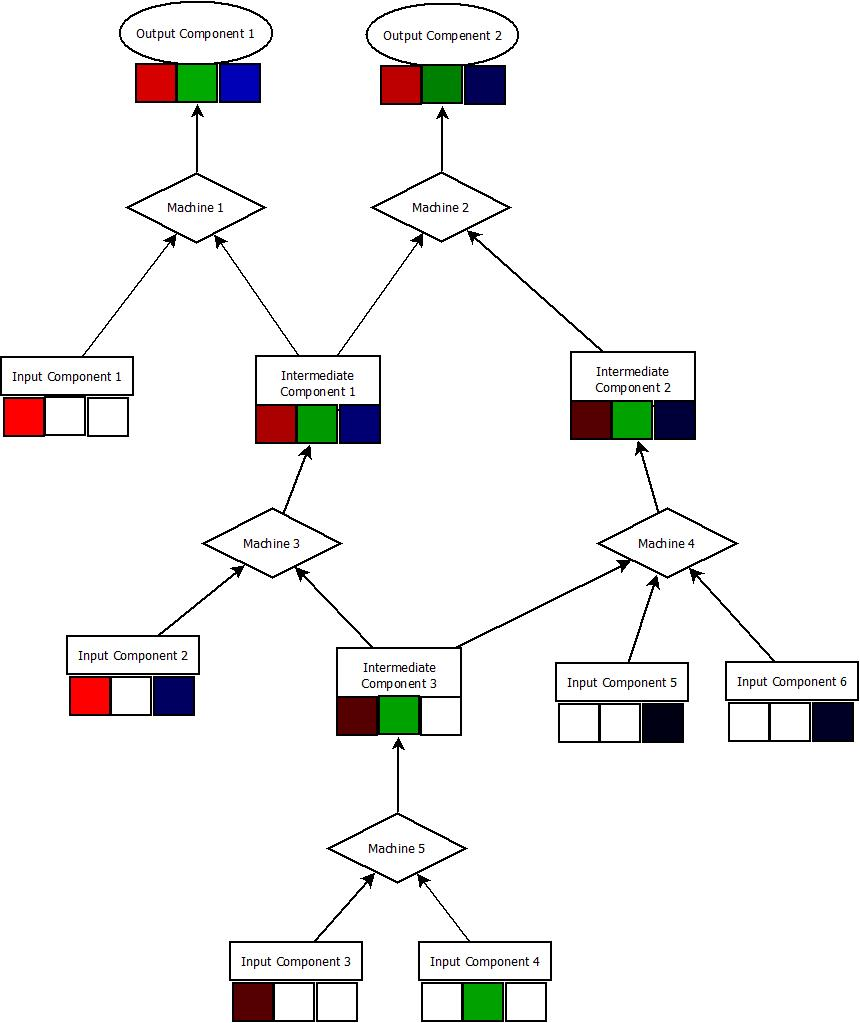
\includegraphics[width=\columnwidth]{Diagram1.jpeg}}
\caption{The above diagram illustrates our modeling approach. Imagine for instance that this example is for creating two types of electrical wire. Red indicates the general durability attribute, green for conductivity, and blue for malleability. The hue indicates a user-defined aspect of a particular component attribute, for instance variation. A darker color designates a lower value, for instance less variation, which is typically associated with higher quality. The different color hues in the diagram demonstrate some of the possible attribute-transformation-interactions, where nonlinear effects between input attributes may translate to the output attributes.}
\label{fig1}
\end{figure}

\section{EC Background}
\subsection{GP Background}

\subsection{EA Background}

\subsection{MOEA Background}

\section{Methodology}
\subsection{Part-DNA Model}
We designed our Part-DNA Model on the principle of taking input components and performing some form of transformation on the input components' attributes and producing an output component. The whole process consisting of a set of transformations based on the list of input and intermediate components leading to a final set of output components. For the purposes of testing, we created two subsets of data for the input component attributes and transformation functions:
\begin{enumerate}
\item Randomly generated values to test GP strategies.
\item Hand made values to test MOEA strategies.
\end{enumerate}
We chose these methods to ensure fitness evaluations would more closely resemble a real-world scenario for the application of the designed methods.

\subsection{reword}
In regards to the GP problem,

As for the MOEA portion, in a real world scenario; the input parameters, as well as intermediate and ouput parameters should be well documented and proper domain and range knowledge

\subsection{GP}
For this problem, we used a binary tree representation to generate our goal functions and to evolve approximations to those functions. We generated leaf nodes from one of the following groups: one of the attributes from any input component, or a constant number, real valued or discrete. Non-leaf nodes used the addition, subtraction, and multiplication operands. For testing the accuracy of the evolved solutions, the fitness was calculated as the sum squared error (SSE) across 64 combinations of input components with an addition of max tree depth to encourage consice representations.
\begin{equation} \label{eq:1}
\begin{split}
fitness=(penaltyfactor)*treedepth \\
+ \sum (expected-result)^{2}
\end{split}
\end{equation}
%Equation \ref{eq:1} shows the fitness function written out.

\subsection{MOEA}
For this problem, we created a model that used three transformation sets (machines) and four types of input components, with each component have four sub-types. The solution is represented as a sub-type selection for each input type. Each solution is rated based on how close it is to the goal component and how much each input selection cost.

\section{Results}
\subsection{Sample GP models}
We tested this model on random functions up to depth four and a randomly generated set of 64 input components. Up to depth three, on average half of the transformation functions were modeled accurately with 75 generations. At depth four, average approximations had an SSE value less than 16, or .25 units away per input combination.

\subsection{MOEA solutions}
\begin{figure}[!t]
\centerline{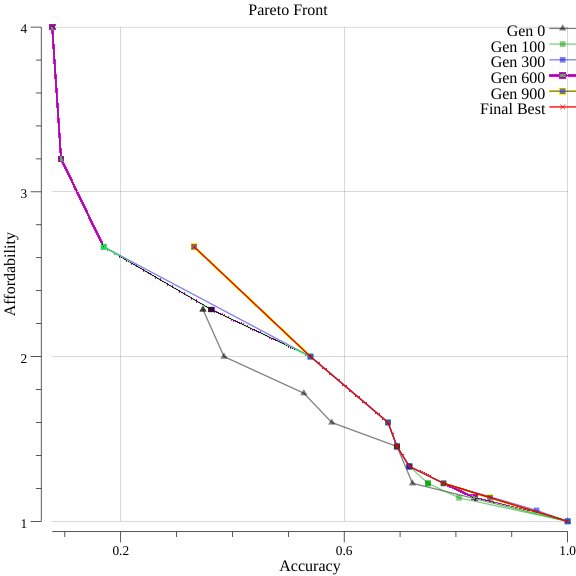
\includegraphics[width=\columnwidth]{points.png}}
\caption{The above diagram shows a Pareto Front graph which plots the set of optimal trade-off points. None of the points shown are entirely better than any other point on the graph. The top-right point has the best accuracy, but also has the highest cost. The bottom-left point is the opposite, having the lowest accuracy and cost. Both options have a benfit over the others.}
\end{figure}

\section{Future Work}
A natural extension of the proposed work is to simultaneously with the proposed trade-off optimization, also optimize the organization of all the different machines in the plant based on their individual processing times, in order to achieve maximum efficiency. The latter is an instance of the general Job Shop Scheduling problem.

\begin{thebibliography}{00}
\bibitem{b1} https://www.youtube.com/watch?v=cc16ClXGuYQ
\end{thebibliography}

\end{document}